\chapter{Methods}
\label{cha:methods}

This chapter describes the background of the developed interface for integrating several drug related knowledge bases.
The project is called Semantic Drug Interface (SEDRI) and will be explained by the following sections in detail.

\section{Data integration}
\label{sec:data-integration}

Before the architecture and used data sets of SEDRI will be explained, this section will discuss the different possibilities of integrating semantic data sets.

At first there is a distinction between virtual and local (also: materialized) integration \cite{lenzerini2002data}.
Virtual integration means that several federated data sets are queried and the results will be integrated virtually at query time independently of the source data sets.
In contrast, the local integration deploys an own copy of the data sets locally and integrates them based on certain criteria.
The main criteria that decides which approach is more suitable are query performance versus currentness of the data.

Virtual integration provides always up-to-date data because the knowledge bases are queried directly.
In the majority of cases this also leads to slower query times compared to local integration.
This is naturally caused by network times and the delay of the integration process.
Additionally it is not uncommon that knowledge bases are not available for a given time.

The local integration approach only queries a local target and therefore it is more performant in most of the cases.
The downside of this approach is that the data has to be updated regularly or the integration component will provide outdated data very quickly.

Example engines for the virtual integration of semantic knowledge bases are SPARQL~1.1 federated queries or tools like FedX \cite{schwarte2011fedx} that support also SPARQL < 1.1.
With SPARQL 1.1 it is possible to query multiple tagets with one statement by using the \texttt{SERVICE} keyword.
Listing \ref{lst-fed} gives an example of a federated query over two knowledge bases.

\lstset{language=sparql}
\begin{lstlisting}[label=lst-fed,numbers=none,caption=Example of SPARQL 1.1 federated query]
PREFIX foaf: <http://xmlns.com/foaf/0.1/>

SELECT ?name
FROM <http://example.org/myfoaf.rdf>
WHERE
{
  <http://example.org/myfoaf/I> foaf:knows ?person .
  SERVICE <http://people.example.org/sparql> { 
    ?person foaf:name ?name . } 
}
\end{lstlisting}

These federated queries are an easy yet powerful way to perform queries over multiple knowledge bases without the use of external tools.
The only problem is that the specific endpoints have to support SPARQL 1.1 which is currently not given in all cases.

An example of a local integration is the Linked Life Data project.\footnote{Linked Life Data: \url{http://linkedlifedata.com} (last access Sep 04, 2013)}
This project integrates multiple knowledge bases like Drugbank or Diseasome.
A disadvantage of the project is the license model\footnote{Linked Life Data -- license model: \url{http://linkedlifedata.com/about} (last access Sep 04, 2013)} which states that free access is limited to only one query per 30 seconds and only annual updated data sets.
Otherwise the commercial enterprise license is required which then would allow umlimited query execution and monthly updated data sets.

Which approach the SEDRI project uses will be explained in the following section.

\section{Architecture}
\label{sec:architecture}

As figure \ref{fig:arch_sedri} shows, the Semantic Drug Interface acts like an abstraction and integration layer between the source data and the end user applications.

\begin{figure}
  \centering
  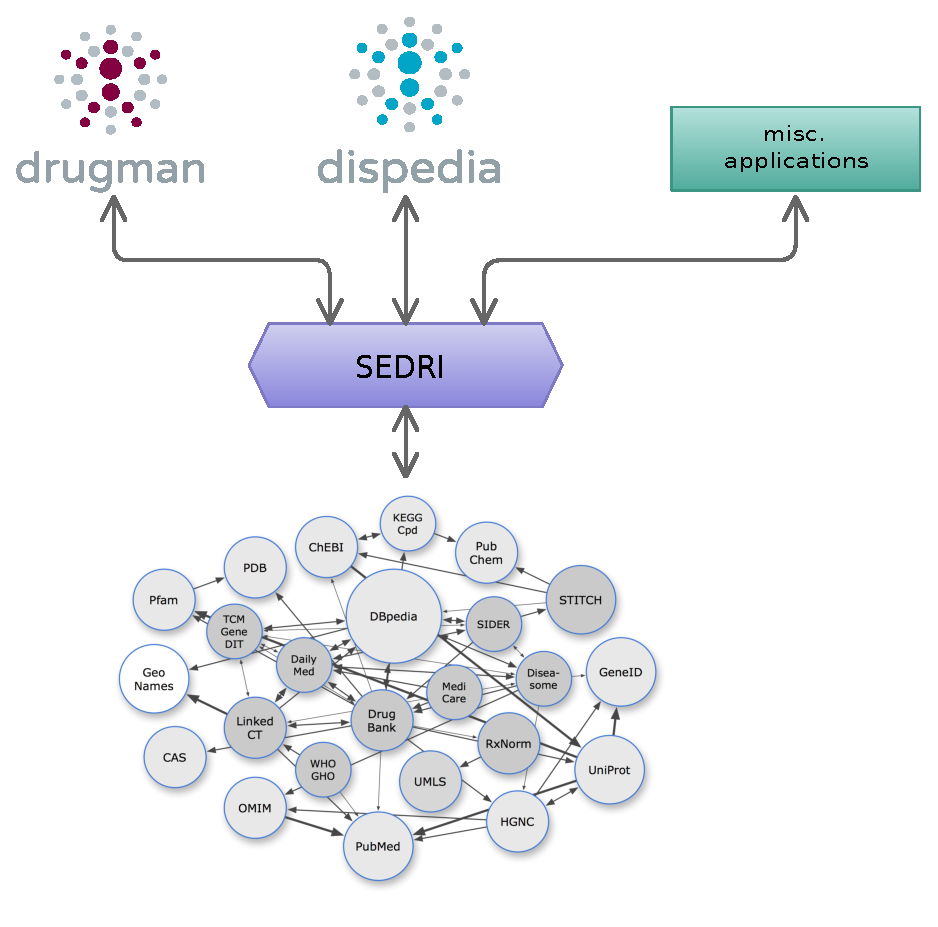
\includegraphics[scale=0.7]{methods/wrapper2.eps}
  \caption{Overview of the SEDRI infrastructure}
  \label{fig:arch_sedri}
\end{figure}
Section \ref{sec:data-integration} described the different possible approaches for integrating semantic knowledge bases.
SEDRI currently uses a virtual integration approach.
The reasons for this decision is the simplicity, the low costs of the approach and the fact that possible applications expect always up-to-date knowledge.
Especially in the biomedical domain this is an important requirement.
SEDRI does not use the SPARQL 1.1 federated query possibility because many of the used data sets, or more specific the respectiv SPARQL endpoints, doesn't support this feature yet.
Therefore the different SPARQL endpoints are queried and the results merged.
The results are queried by a SPARQL \texttt{CONSTRUCT} or \texttt{DESCRIBE} statement.
This means that always full RDF resources are returned and not only single entities or literals that are returned by a \texttt{SELECT} query.
These RDF resources can be returned by SEDRI in several representation formats, like \textit{Turtle}, \textit{RDF/XML} or \textit{JSON-LD}.
By default JSON-LD will be returned, because JSON in general is the dominating data exchange format of modern web API's.
Other formats can be requested by setting the HTTP \texttt{Accept} Header to the appropriate MIME type.

To abstract from the required background knowledge about the data sources, SEDRI predefines some API endpoints that are easily usable by only providing the necessary drug codes.
As such drug codes currently the Anatomical Therapeutic Chemical Classification System (ATC) code or the Drugbank ID are supported.
These IDs are required to identify a drug unambigiously.
The API endpoints are designed to cover each phase of the WHO drug management life cycle.
The following paragraphs describe all available API endpoints that are provided by SEDRI and the respective SPARQL queries and show an example request for each endpoint.

\subsection*{Drug-drug interactions}
This endpoint expects at least two drug codes and checks these drugs for possible drug-drug interactions.
In detail each possible combination of the given drugs is calculated and tested for interactions.
The maximum number of drug codes is unlimited.
This use case is mainly placed in the \textit{Selection} phase of the WHO drug management life cycle.
Here it may help the respective parties, e.g. a physician or pharmacist to prevent that they prescribe drugs that possibly cause harm.\\
The following code listings show example queries to retrieve the interactions of Ibuprofen and Metoprolol as well as in the first example additionally Metoprolol and Bisoprolol.
\begin{lstlisting}[caption=Example Drugbank query for drug-drug interactions between Ibuprofen~--~Metoprolol and Bisoprolol -- Metoprolol]
PREFIX db:  <http://bio2rdf.org/drugbank:>
PREFIX dbv: <http://bio2rdf.org/drugbank_vocabulary:>

DESCRIBE ?ddi
WHERE {
  ?ddi a dbv:Drug-Drug-Interaction .
  
  {
    db:DB01050 dbv:ddi-interactor-in ?ddi .
    db:DB00264 dbv:ddi-interactor-in ?ddi .
  }
  UNION
  {
    db:DB00612 dbv:ddi-interactor-in ?ddi .
    db:DB00264 dbv:ddi-interactor-in ?ddi .
  }
}
\end{lstlisting}
\begin{lstlisting}[caption=Example DIKB query for drug-drug interactions between Ibuprofen and Metoprolol]
PREFIX dikbD2R: <http://dbmi-icode-01.dbmi.pitt.edu:2020/vocab/resource/>
PREFIX dbv:     <http://bio2rdf.org/drugbank_vocabulary:>
PREFIX owl:     <http://www.w3.org/2002/07/owl#>
PREFIX rdfs:    <http://www.w3.org/2000/01/rdf-schema#>

CONSTRUCT {
  ?s a dbv:Drug-Drug-Interaction.
  ?s rdfs:label ?desc.
  ?drug1 dbv:ddi-interactor-in ?s.
  ?drug2 dbv:ddi-interactor-in ?s.
}
WHERE {
  ?s rdfs:label ?desc.
  {
    ?drug1 owl:sameAs db:DB01050 .
    ?drug2 owl:sameAs db:DB00264 .
    {
      ?s dikbD2R:ObjectDrugOfInteraction ?drug1.
      ?s dikbD2R:PrecipitantDrugOfInteraction ?drug2.
    } UNION {
      ?s dikbD2R:ObjectDrugOfInteraction ?drug2.
      ?s dikbD2R:PrecipitantDrugOfInteraction ?drug1.
    }
  }
}
\end{lstlisting}
Listing \ref{lst:ddi} shows an examplary HTTP request url for the drug-drug interaction endpoint.
\begin{lstlisting}[label=lst:ddi,caption=Example request for the drug-drug interaction endpoint]
  GET http://sedri.de/ddi/?drug1=C07AB02&drug2=C07AB07&drug3=C01EB16
\end{lstlisting}

\subsection*{Side effects}
The side effects endpoint expects one drug code and returns all available side effects of this drug.
This component supports primarily the phase \textit{Use} where it could support the treating parties for example if the respective patient shows signs of an adverse effect.
But this component is also applicable for the \textit{Selection}.
In this case drugs with a specific side effect could be excluded.\\
The following code listings show two example queries that retrieve the side effects of Ibuprofen from SIDER and PhramGKB.
\begin{lstlisting}[caption=Example SIDER query for side effects of Ibuprofen]
PREFIX owl: <http://www.w3.org/2002/07/owl#>
PREFIX rdfs: <http://www.w3.org/2000/01/rdf-schema#>
PREFIX sider: <http://wifo5-04.informatik.uni-mannheim.de/sider/resource/sider/>
PREFIX db: <http://wifo5-04.informatik.uni-mannheim.de/drugbank/resource/drugs/>

CONSTRUCT {
  ?se rdfs:label ?label.
  ?se a ?type.
}
WHERE {
  ?drug owl:sameAs db:DB01050 .
  ?drug sider:sideEffect ?se.
  ?se rdfs:label ?label.
  ?se a ?type.
}
\end{lstlisting}
\begin{lstlisting}[caption=Example PharmGKB query for side effects of Ibuprofen that are not listed in SIDER]
PREFIX pharmgkbv:  <http://bio2rdf.org/pharmgkb_vocabulary:>

CONSTRUCT {
  ?side rdfs:label ?label.
  ?side pharmgkbv:p-value ?p.
  ?side a pharmgkbv:Side-Effect.
  ?side pharmgkbv:event ?event.
}
WHERE {
  ?drug pharmgkbv:xref <http://bio2rdf.org/drugbank:DB01050>.
  ?drug pharmgkbv:xref ?chem.
  ?side pharmgkbv:chemical ?chem.
  ?side a pharmgkbv:Side-Effect.
  ?side pharmgkbv:in-sider "false".
  ?side pharmgkbv:event ?event.
  ?side pharmgkbv:p-value ?p.
  ?event rdfs:label ?label.
}
\end{lstlisting}
Listing \ref{lst:sides} shows an examplary HTTP request url for the side effects endpoint.
\begin{lstlisting}[label=lst:sides,caption=Example request for the side effects endpoint]
  GET http://sedri.de/sideeffects/?drug=C07AB02
\end{lstlisting}

\subsection*{Procurement}
The procurement component returns the possible manufacturers and packagers for a given drug code.
Trivialy this component supports the \textit{Procurement} phase of the drug management life cycle.

\begin{lstlisting}[caption=Example Drugbank query for procurement meta data of Ibuprofen]
PREFIX dbv: <http://bio2rdf.org/drugbank_vocabulary:>
PREFIX db: <http://bio2rdf.org/drugbank:>

CONSTRUCT {
  db:DB01050 dbv:packager ?packager.
  ?packager ?p ?o.
  db:DB01050 dbv:manufacturer ?manufacturer.
}
WHERE {
  db:DB01050 dbv:packager ?packager.
  ?packager ?p ?o.
  db:DB01050 dbv:manufacturer ?manufacturer.
}
\end{lstlisting}
Listing \ref{lst:proc} shows an examplary HTTP request url for the procurement endpoint.
\begin{lstlisting}[label=lst:proc,caption=Example request for the procurement endpoint]
  GET http://sedri.de/procure/?drug=C07AB02
\end{lstlisting}

\subsection*{Drug proposals}
This endpoint proposes several drugs to a given disease.
To specify the disease currently only the Medical Subject Headings (MeSH) ID is supported.
As results the respective URIs to the drugs are returned.
With these URIs more details can be retrieved or other endpoints of SEDRI may be used.
This component covers the \textit{Selection} phase where it could support the physician by chosing an appropriate drug to a given disease.
Important is the fact that these are only recommendations to relieve the physiscian -- the final decisision has to be made by the expert.

In example \ref{lst:diseasome} \texttt{diseasome:561} is the appropriate Diseasome URI of ``Hypertension'' which was converted from the MeSH ID (D006973) by DBpedia in a previous request.

\begin{lstlisting}[caption=Example Diseasome query for possible drugs of Hypertension,label=lst:diseasome]
PREFIX diseasome <http://www4.wiwiss.fu-berlin.de/diseasome/resource/diseases/>

CONSTRUCT {
  diseasome:561 diseasome-instance:possibleDrug ?o.
}
WHERE {
  diseasome:561 diseasome-instance:possibleDrug ?o.
}
\end{lstlisting}
Listing \ref{lst:prop} shows an examplary HTTP request url for the drug proposal endpoint.
\begin{lstlisting}[label=lst:prop,caption=Example request for the drug proposal endpoint]
  GET http://sedri.de/proposal/?code=D006973
\end{lstlisting}

\subsection*{Pharmacokinetic meta data}
This component returns several meta data for a given drug code.
The results contains mainly pharmacokinetic information like dosages, the affected organism or the route of elimination.
In the WHO drug management life cycle this component covers mainly the \textit{Use} phase but also in parts the \textit{Selection} phase.

\begin{lstlisting}[caption=Example Diseasome query for possible drugs of Hypertension,label=lst:diseasome]
PREFIX db: <http://bio2rdf.org/drugbank:>
PREFIX dbv: <http://bio2rdf.org/drugbank_vocabulary:>
PREFIX dc: <http://purl.org/dc/terms/>

CONSTRUCT {
  db:DB01050 dbv:absorption ?absorption.
  db:DB01050 dbv:affected-organism ?organism.
  db:DB01050 dbv:dosage ?dosage.
  ?dosage rdfs:label ?dosage_label.
  db:DB01050 dbv:food-interaction ?food.
  db:DB01050 dbv:indication ?indication.
  db:DB01050 dbv:mechanism-of-action ?mechanism.
  db:DB01050 dbv:route-of-elimination ?elimination.
  db:DB01050 dc:description ?description.
}
WHERE {
  db:DB01050 dbv:absorption ?absorption.
  db:DB01050 dbv:affected-organism ?organism.
  db:DB01050 dbv:dosage ?dosage.
  ?dosage rdfs:label ?dosage_label.
  db:DB01050 dbv:food-interaction ?food.
  db:DB01050 dbv:indication ?indication.
  db:DB01050 dbv:mechanism-of-action ?mechanism.
  db:DB01050 dbv:route-of-elimination ?elimination.
  db:DB01050 dc:description ?description.
}
\end{lstlisting}
%The appropriate SPARQL query omitted due to its extent and simplicity.
Listing \ref{lst:meta} shows an examplary HTTP request url for the meta data endpoint.
\begin{lstlisting}[label=lst:meta,caption=Example request for the meta data endpoint]
  GET http://sedri.de/details/?drug=C07AB02
\end{lstlisting}

\newpage
\section{Data sets}
\label{sec:data-sets}

The following Table gives an overview of the data sets that are used by SEDRI for the different API endpoints.
The table also contains a short description of the data set and how it is used by SEDRI.

% \begin{itemize}
% \item übersicht datensätze
%   \begin{itemize}
%   \item tabellarisch/grafisch
%   \item proprietäre quellen die nicht verwendet werden konnten
%     \begin{itemize}
%     \item senger et al
%     \end{itemize}
%   \end{itemize}
% \end{itemize}

\begin{longtable}{p{\textwidth/4}|p{\textwidth/3}|p{\textwidth/3}}
  Data set & Description & Usage\\
  \hline
  DBpedia & DBpedia retrieves meta data form Wikipedia pages that are often shown in info boxes. DBpedia therefore provides many cross domain information and takes a central role in the Linked Open Data cloud. In 2011 DBpedia contained descriptions about more than 3.64 million things including 5,400 diseases. & The data set is used for converting the given ATC codes of drugs to Drugbank IDs for a better processing. The second use case is the proposal endpoint where DBpedia is used for the assignment of the Diseasome URI to a given MeSH code.\\
  Drugbank & Drugbank is a large knowledge base that contains many different information about drugs and their meta data such as interactions, dosages or manufacturers. It has a comparable central role like DBpedia but in the biomedical part of the Linked Open Data cloud. & Drugbank is the main knowledge base used by SEDRI. It provides information for nearly each given endpoint, except the side effects.\\
  SIDER & The main domain of SIDER are adverse drug reactions. ``The information is extracted from public documents and package inserts''\footnote{\url{http://sideeffects.embl.de/} (last access Sept 19, 2013)} and includes ``side effect frequency, drug and side effect classifications as well as links to further information, for example drug–target relations''. & SIDER is only used by the side effects endpoint.\\
  Drug Interaction Knowledge Base (DIKB) & The DIKB is an evidence-focused knowledge base that provides information about drug drug interactions. ``The DIKB contains quantitative and qualitative assertions about drug mechanisms and pharmacokinetic drug-drug interactions''\footnote{\url{http://dbmi-icode-01.dbmi.pitt.edu/dikb-evidence/front-page.html} (last access Sept 09, 2013)} & DIKB is used as additional source for the interactions endpoint.\\
  Pharmaco\-genomics Knowledge Base (PharmGKB) & ``PharmGKB curates primary genotype and phenotype data, annotates gene variants and gene-drug-disease relationships via literature review, and summarizes important PGx genes and drug pathways.''\cite{hewett2002pharmgkb} & PharmGKB is used as additional source for the side effects endpoint.\\
  Diseasome & ``[...] Diseasome publishes a network of 4,300 disorders and disease genes linked by known disorder-gene associations for exploring all known phenotype and disease gene associations, indicating the common genetic origin of many diseases. The list of disorders, disease genes, and associations between them was obtained from the Online Mendelian Inheritance in Man (OMIM) [...]''\footnote{\url{http://diseasome.eu/about.html} (last access Sept 09, 2013)} & Diseasome is used for proposing drugs to a given disease implemented in the proposals endpoint.\\
\hline
\caption{Description and usage of the relevant SEDRI data sets}
\end{longtable}

%%% Local Variables: 
%%% mode: latex
%%% TeX-master: "../thesis"
%%% End: 
